\documentclass[journal,12pt,onecolumn]{IEEEtran}
\usepackage{mathtools,amssymb,amsfonts}
\usepackage{algorithmic}
\usepackage{algorithm}
\usepackage{graphicx}
\usepackage{xcolor}
\usepackage{float}
\usepackage{setspace}
\usepackage{subcaption}
\usepackage[hidelinks]{hyperref}
\usepackage{multirow}

\doublespacing

\hypersetup{
   colorlinks=true,
   linkcolor=blue,
   citecolor=black,
   urlcolor=blue
}

\usepackage{titlesec}
\titlespacing*{\section}{0pt}{12pt plus 4pt minus 2pt}{12pt plus 2pt minus 2pt}
\titlespacing*{\subsection}{0pt}{12pt plus 4pt minus 2pt}{8pt plus 2pt minus 2pt}
\titlespacing*{\subsubsection}{0pt}{12pt plus 4pt minus 2pt}{6pt plus 2pt minus 2pt}

\title{Genetic Algorithm: Bin Packing Problem}
\author{
   \IEEEauthorblockN{Matthew D. Branson} \\
   \IEEEauthorblockA{\textit{Department of Computer Science} \\
   \textit{Missouri State University}\\
   Springfield, MO \\
   branson773@live.missouristate.edu
   }
}

\date{July 5, 2025}

\begin{document}

\maketitle

\begin{abstract}
This paper presents the implementation and analysis of a...
\end{abstract}

\begin{IEEEkeywords}
Genetic Algorithms, Bin Packing Problem, Optimization, Heuristic Search
\end{IEEEkeywords}

\section{Q1: Encoding and Initialization}

An integer-based representation is used to encode bin assignments. For an instance with $N$ items, each individual is a vector of length $N$, where the value at index $i$ denotes the bin to which item $i$ is assigned.

For example, the encoding \texttt{[0, 1, 0, 2, 1, 1, 2, 1, 3, 0]} represents a solution for 10 items in which items 0, 2, and 9 are assigned to bin 0; items 1, 4, 5, and 7 to bin 1; items 3 and 6 to bin 2; and item 8 to bin 3, resulting in the use of 4 unique bins.

Initial populations are generated by assigning each item independently to a random bin in the range $[0, N-1]$. This produces diverse initial solutions while satisfying the constraint that the maximum number of bins does not exceed the number of items.

\section{Q2: Function Evaluation}

\subsection{Objective Function}

The objective function $f$ measures the number of unique bins used in a given individual. For instance, the encoding \texttt{[0, 1, 0, 2, 1, 1, 2, 1, 3, 0]} uses bins \{0, 1, 2, 3\}, yielding $f = 4$. The algorithm minimizes $f$ to reduce the total number of shipping boxes required.

\subsection{Constraint Handling}

The constraint violation function $g$ counts the number of bins whose total weight exceeds the 10 kg capacity. For each bin, the weights of assigned items are summed. A bin contributes 1 to $g$ if its cumulative weight exceeds the limit. A solution is considered feasible when $g = 0$.

\subsection{Evaluation Function}

Each individual is evaluated as a tuple $(f, g)$, where $f$ represents the number of bins used and $g$ the number of constraint violations. This formulation enables the algorithm to balance minimization of bin usage with satisfaction of feasibility constraints.


\section{Q3: GA Operations}

\subsection{Tournament Selection}

Tournament selection is used to construct a mating pool of $N$ individuals. For each selection, two candidates are drawn at random, and the winner is determined by a constraint-aware comparison rule. This process is repeated $N$ times. Mating pairs are then selected at random from the resulting pool.

\subsection{Winner Selection Rules}

Selection is guided by the following criteria:
\begin{itemize}
    \item If both individuals are feasible ($g_1 = 0$, $g_2 = 0$), the one with lower $f$ is preferred.
    \item If only one is feasible, the feasible individual is selected.
    \item If both are infeasible, the one with fewer violations ($g$) is selected.
\end{itemize}

These rules guide selection toward feasible individuals with fewer bins and penalize constraint violations when feasibility is not yet achieved.

\subsection{Crossover}

Two-point crossover is applied with a probability of 0.9. Two cut points are chosen to divide each parent chromosome into three segments. Offspring are generated by exchanging the middle segments, preserving the integer-based encoding and promoting genetic diversity.

\subsection{Mutation}

Each gene (bin assignment) is mutated independently with probability $p_m = 1/N$, where $N$ is the number of items. When selected, a gene is reassigned to a random integer in $[0, N-1]$. This maintains valid encodings while introducing variation for local exploration.

\section{Q4: GA Execution}

\subsection{Baseline Configuration}

The genetic algorithm was initially executed using the specified baseline parameters: population size of 20 and 50 generations. This configuration was tested on four problem instances containing 10, 25, 50, and 100 orders, with order weights uniformly distributed between 0 and 2 kg and a bin capacity of 10 kg.

\subsection{Parameter Variation Study}

To assess the impact of population size and generation count on performance, additional configurations were tested. Population sizes of 10 and 40 individuals were compared against the baseline of 20, while generation counts of 25 and 100 were compared against the baseline of 50. Additionally, each configuration was evaluated across all four problem sizes using three random seeds (42, 773, 2025) to examine performance variability.

\subsection{Fitness Plots}

The evolution of best and average fitness values across generations is shown for various configurations.

% Baseline configuration
\begin{figure}[htbp]
\begin{minipage}{0.48\textwidth}
    \centering
    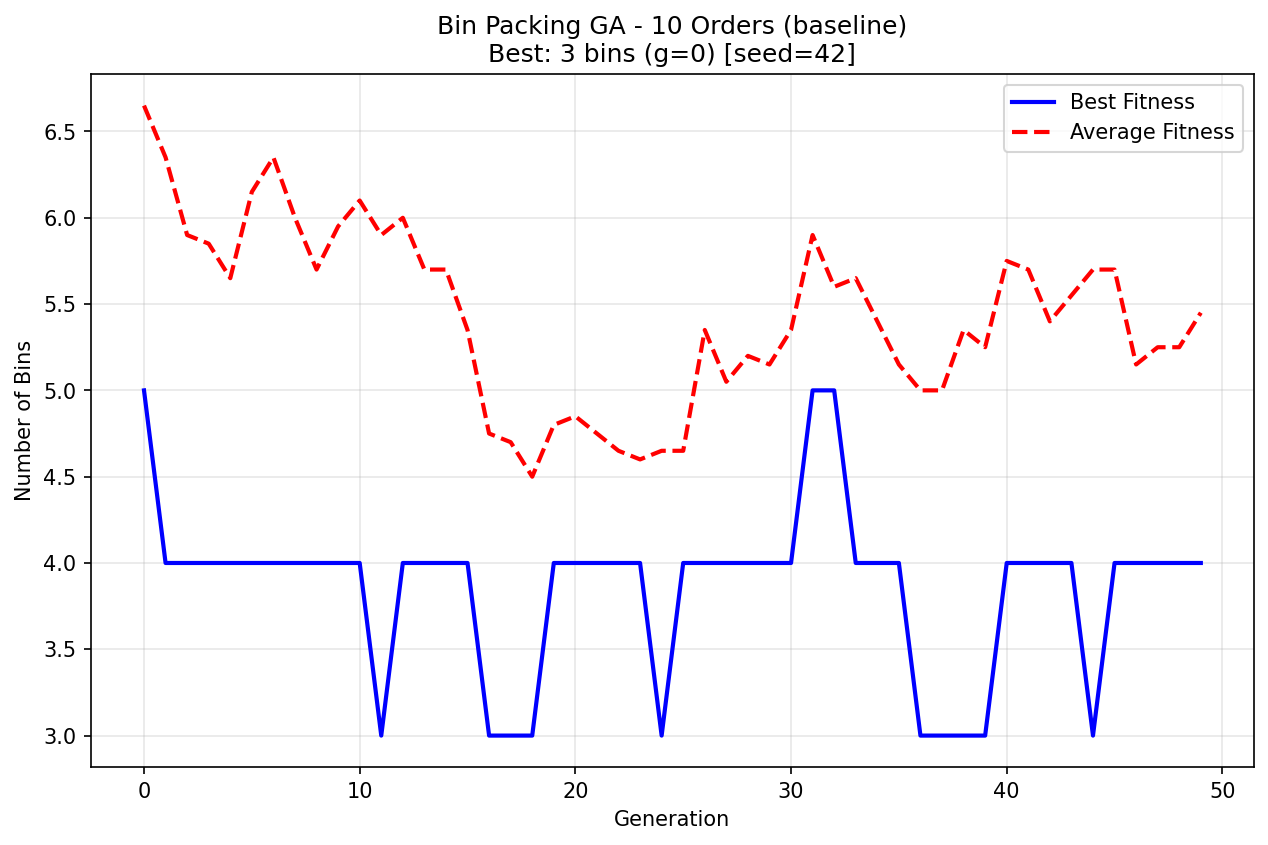
\includegraphics[width=\textwidth]{bpp_10items_baseline_seed42.png}
    \caption{Baseline: 10 orders}
    \label{fig:baseline_10}
\end{minipage}\hfill
\begin{minipage}{0.48\textwidth}
    \centering
    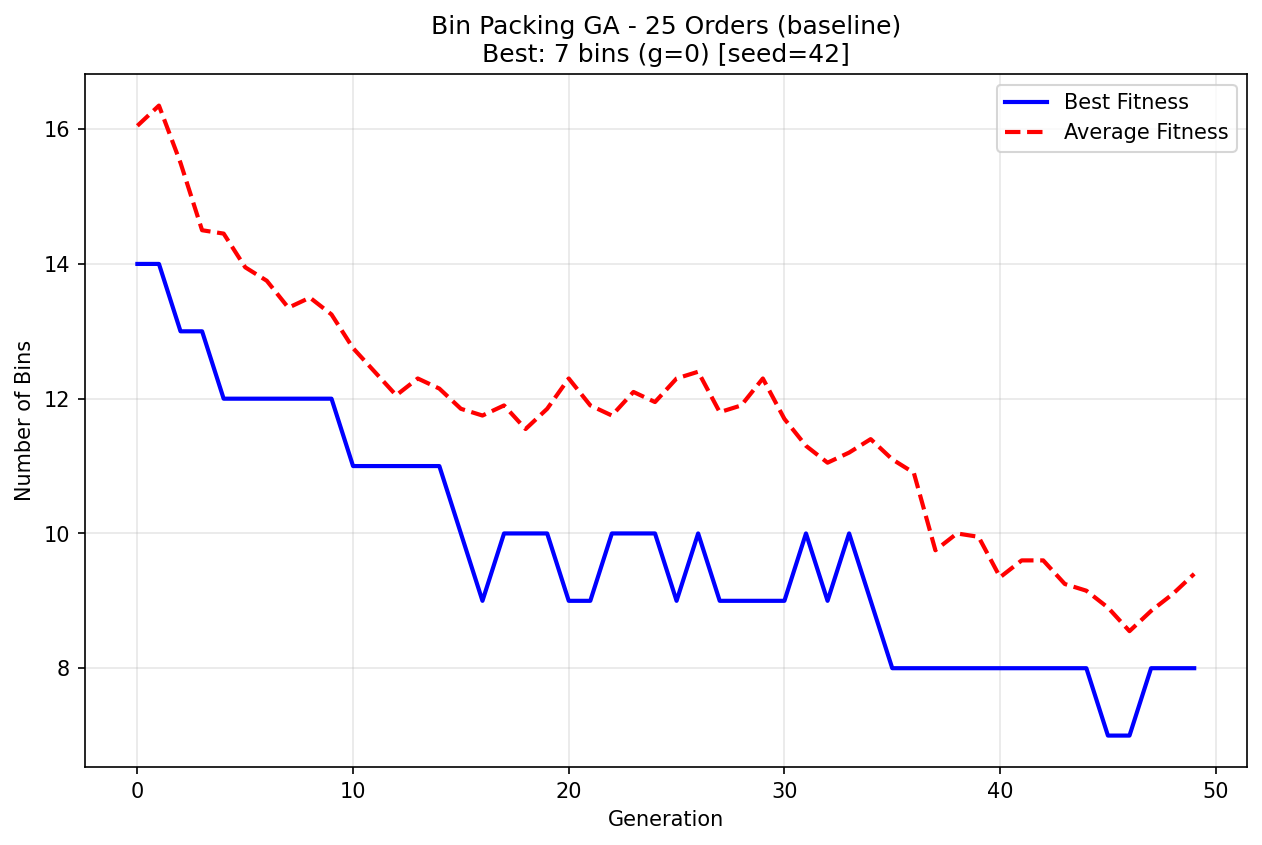
\includegraphics[width=\textwidth]{bpp_25items_baseline_seed42.png}
    \caption{Baseline: 25 orders}
    \label{fig:baseline_25}
\end{minipage}
\end{figure}

\begin{figure}[htbp]
\begin{minipage}{0.48\textwidth}
    \centering
    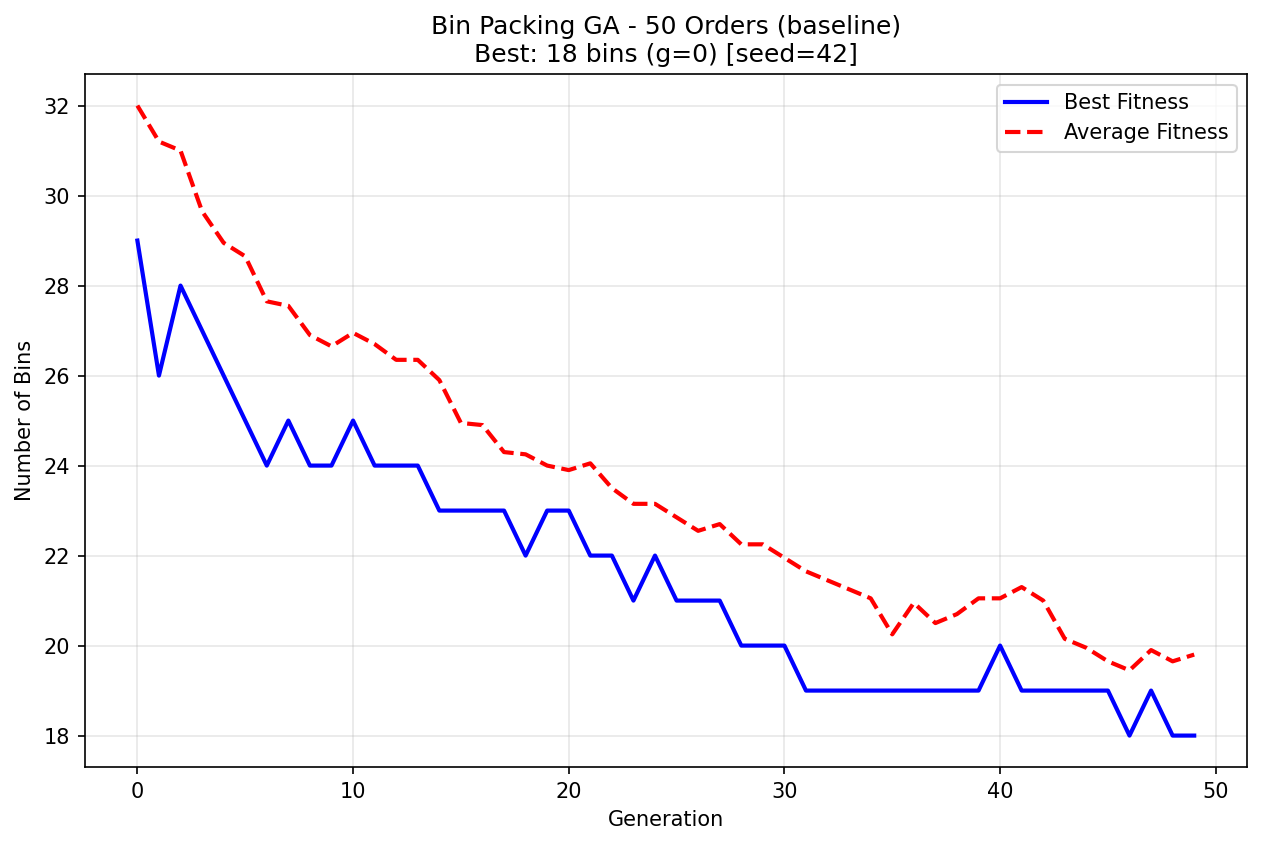
\includegraphics[width=\textwidth]{bpp_50items_baseline_seed42.png}
    \caption{Baseline: 50 orders}
    \label{fig:baseline_50}
\end{minipage}\hfill
\begin{minipage}{0.48\textwidth}
    \centering
    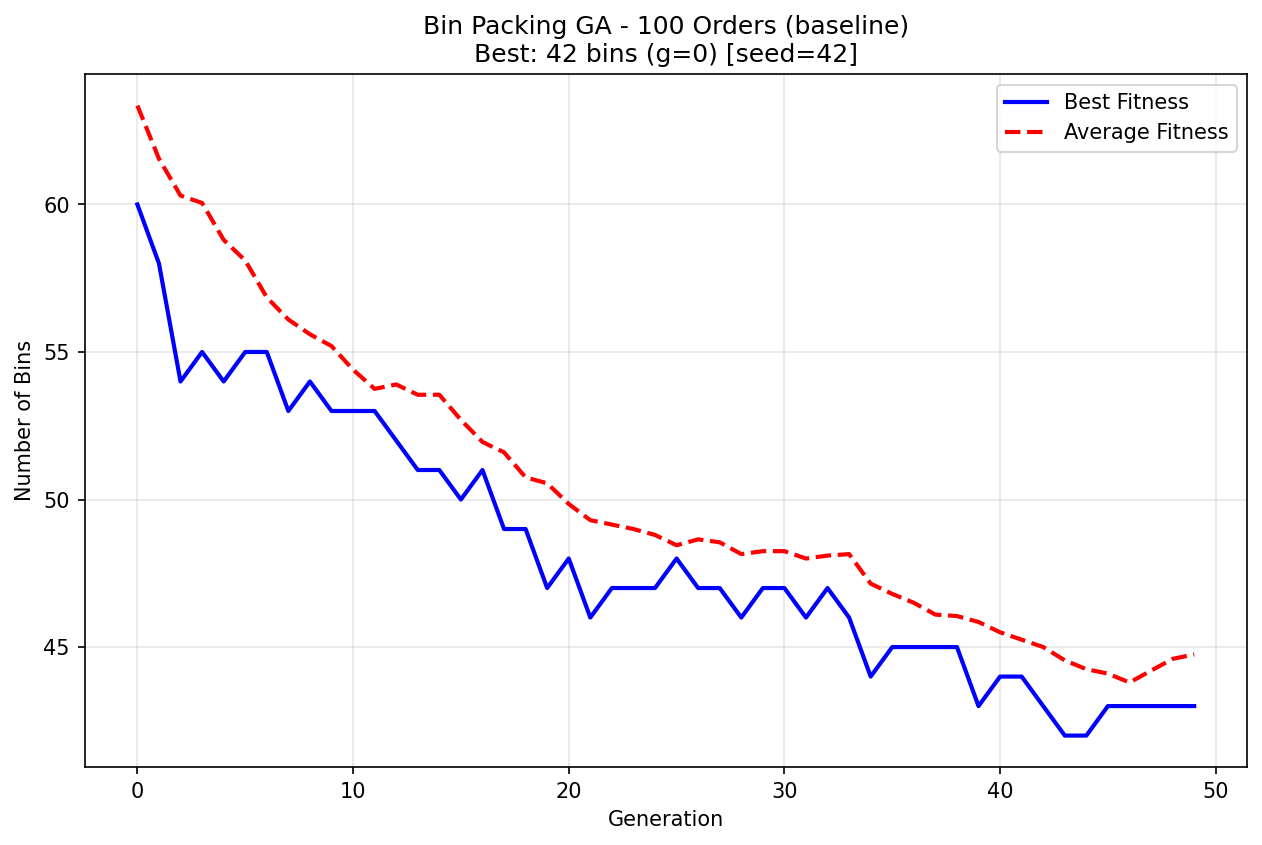
\includegraphics[width=\textwidth]{bpp_100items_baseline_seed42.png}
    \caption{Baseline: 100 orders}
    \label{fig:baseline_100}
\end{minipage}
\end{figure}

% Small population
\begin{figure}[htbp]
\begin{minipage}{0.48\textwidth}
    \centering
    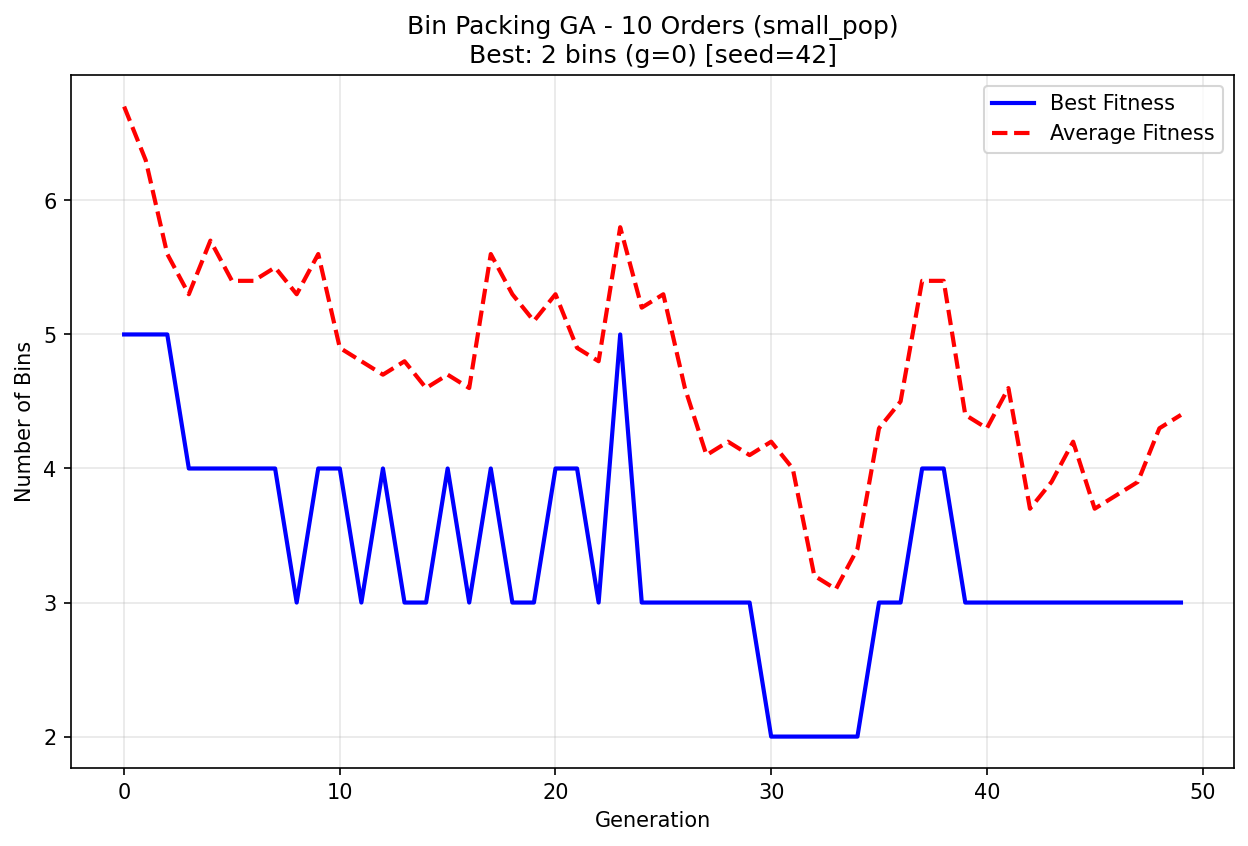
\includegraphics[width=\textwidth]{bpp_10items_small_pop_seed42.png}
    \caption{Small population: 10 orders}
    \label{fig:small_pop_10}
\end{minipage}\hfill
\begin{minipage}{0.48\textwidth}
    \centering
    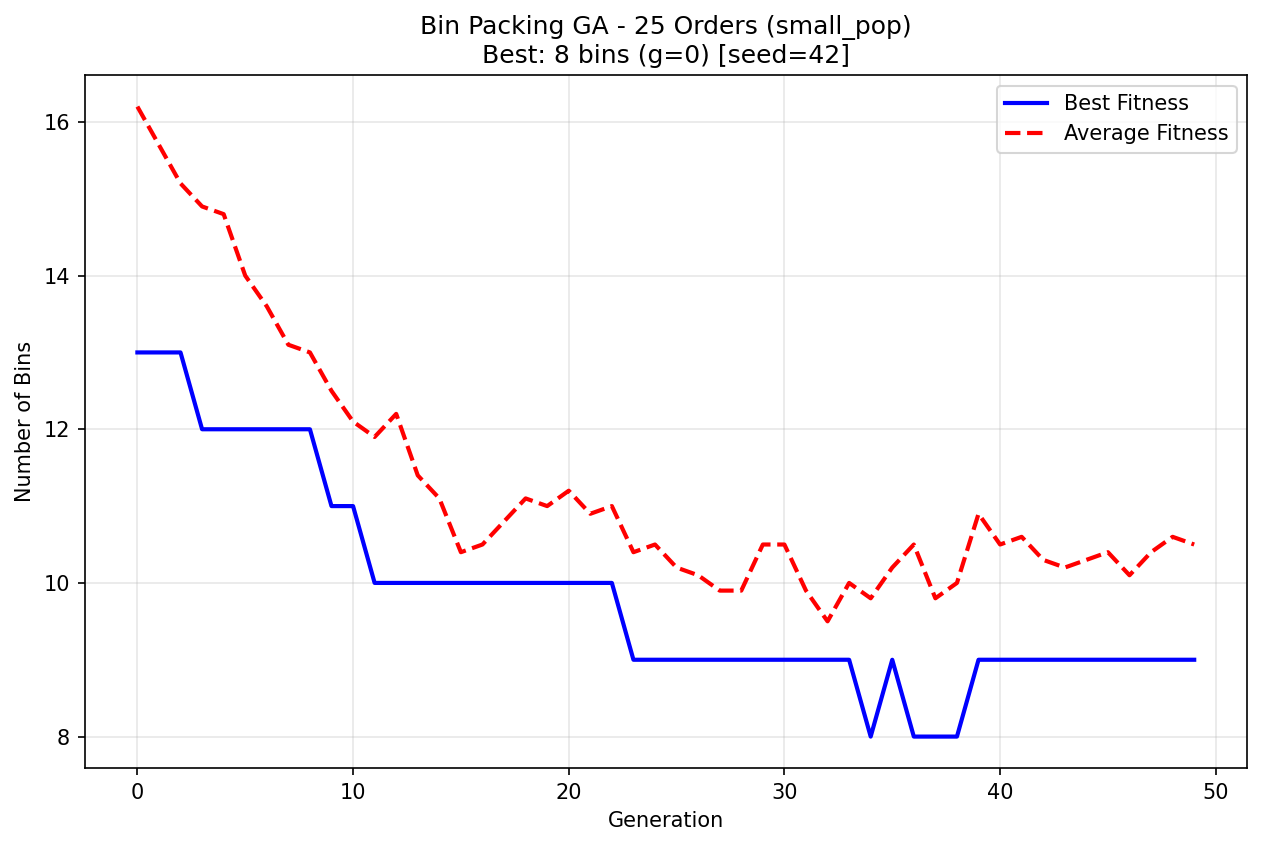
\includegraphics[width=\textwidth]{bpp_25items_small_pop_seed42.png}
    \caption{Small population: 25 orders}
    \label{fig:small_pop_25}
\end{minipage}
\end{figure}

\begin{figure}[htbp]
\begin{minipage}{0.48\textwidth}
    \centering
    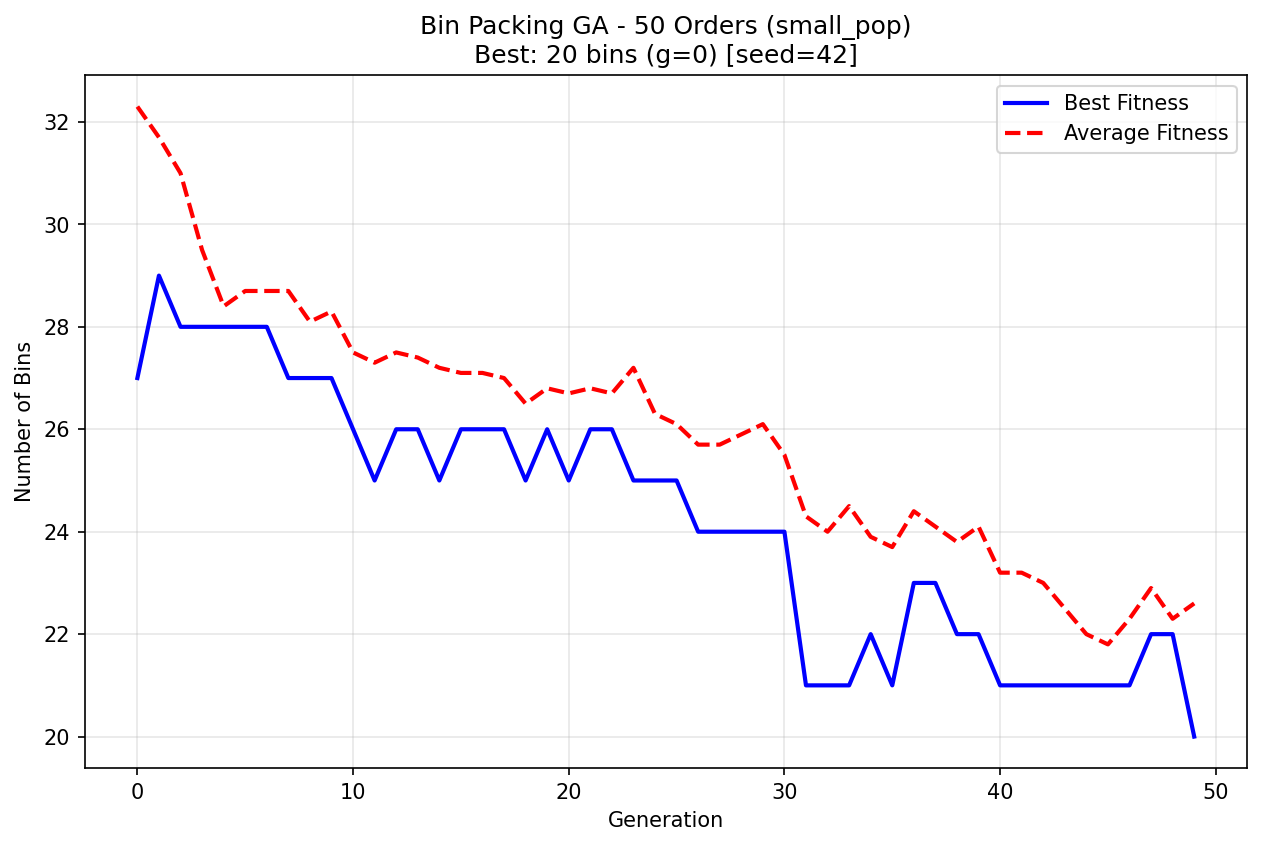
\includegraphics[width=\textwidth]{bpp_50items_small_pop_seed42.png}
    \caption{Small population: 50 orders}
    \label{fig:small_pop_50}
\end{minipage}\hfill
\begin{minipage}{0.48\textwidth}
    \centering
    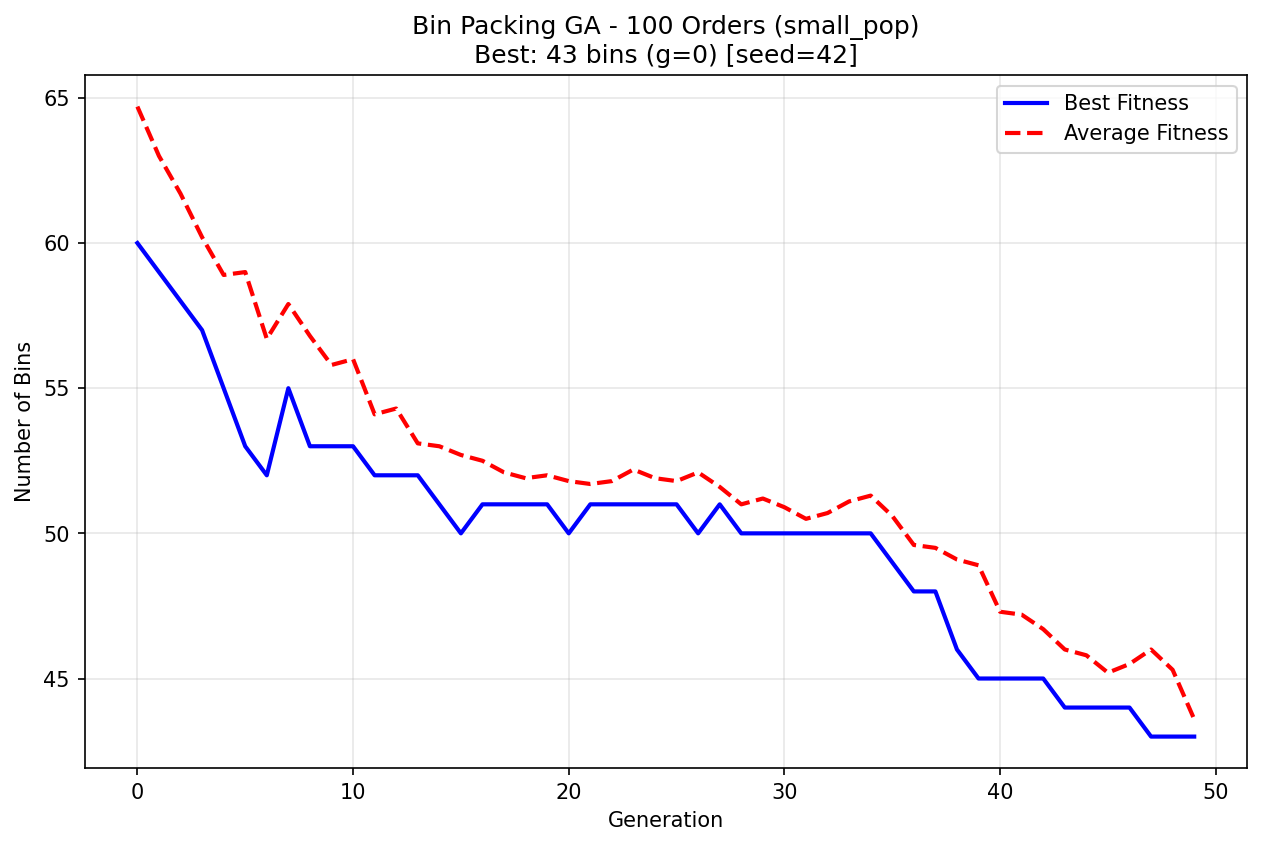
\includegraphics[width=\textwidth]{bpp_100items_small_pop_seed42.png}
    \caption{Small population: 100 orders}
    \label{fig:small_pop_100}
\end{minipage}
\end{figure}

% Large population
\begin{figure}[htbp]
\begin{minipage}{0.48\textwidth}
    \centering
    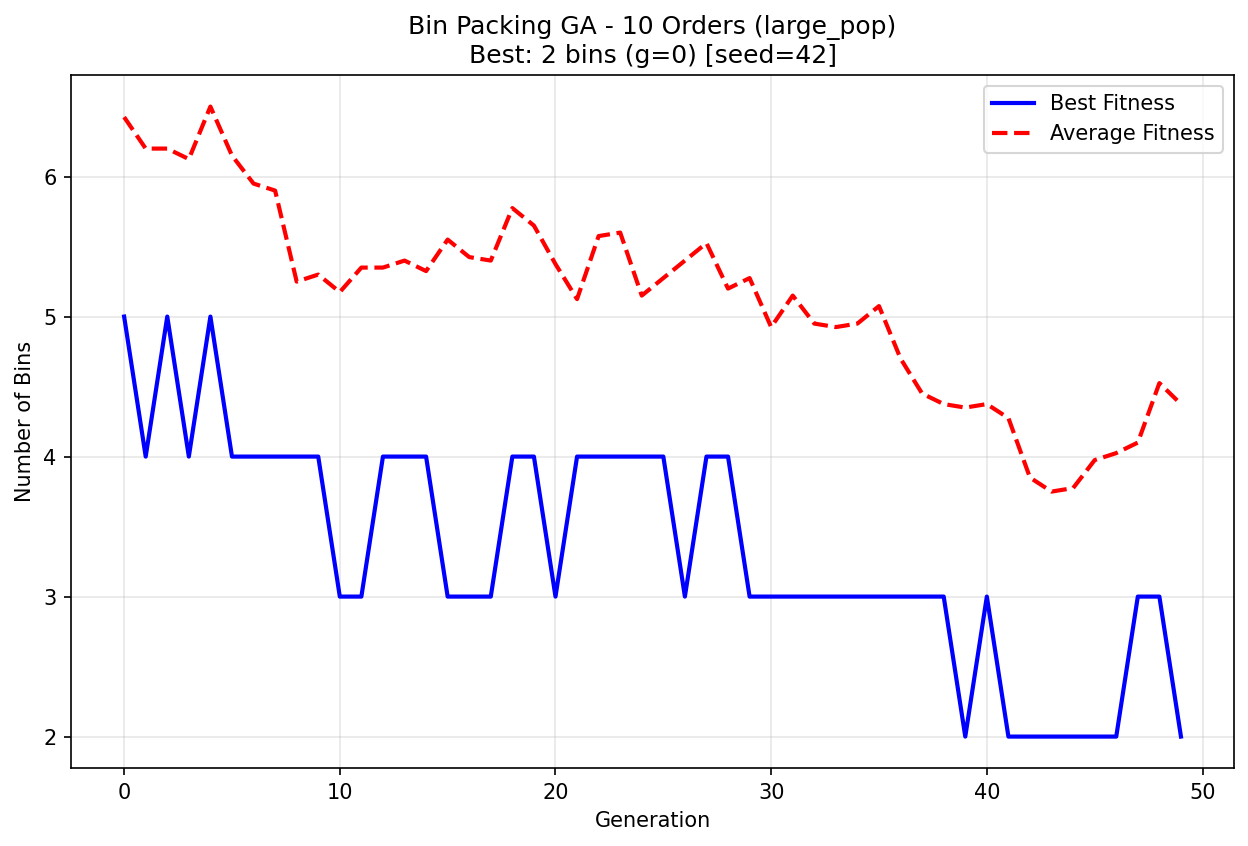
\includegraphics[width=\textwidth]{bpp_10items_large_pop_seed42.png}
    \caption{Large population: 10 orders}
    \label{fig:large_pop_10}
\end{minipage}\hfill
\begin{minipage}{0.48\textwidth}
    \centering
    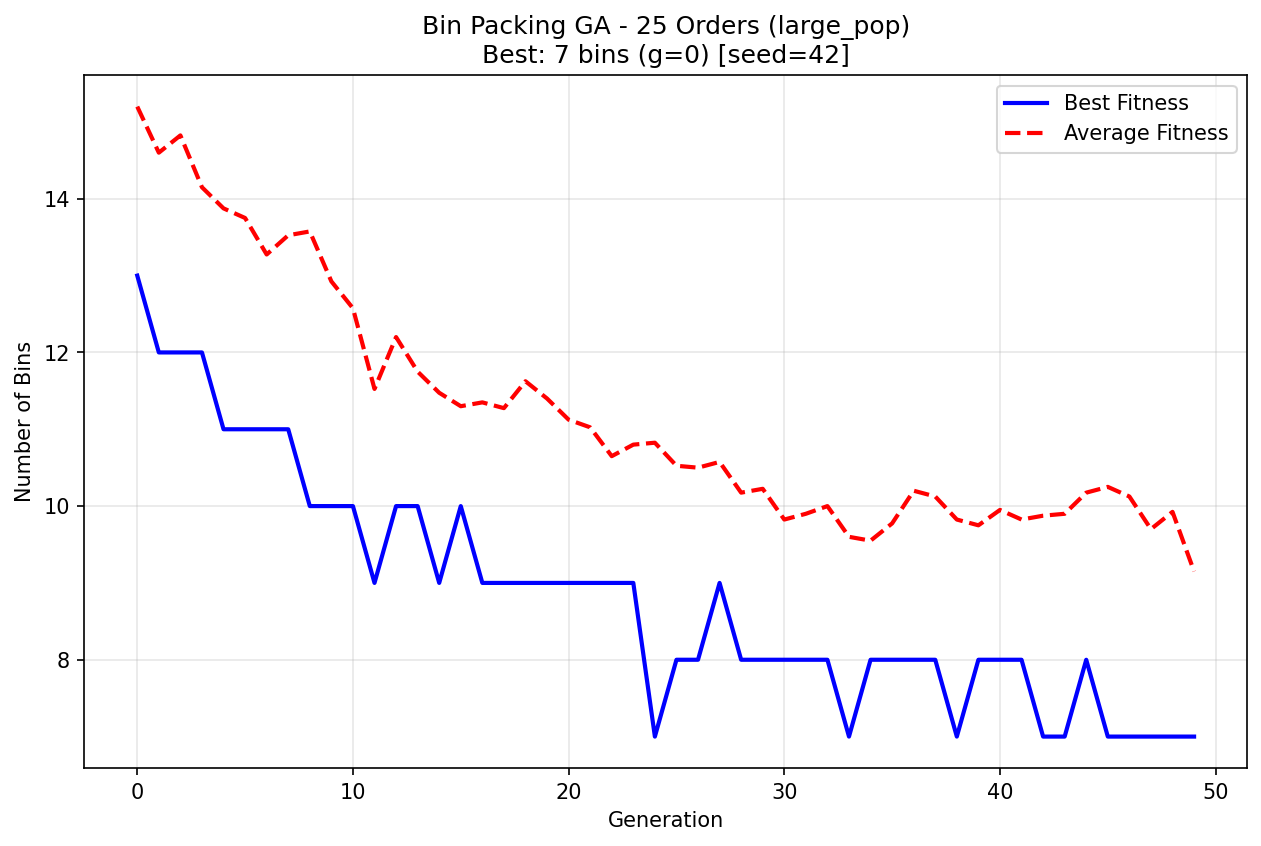
\includegraphics[width=\textwidth]{bpp_25items_large_pop_seed42.png}
    \caption{Large population: 25 orders}
    \label{fig:large_pop_25}
\end{minipage}
\end{figure}

\begin{figure}[htbp]
\begin{minipage}{0.48\textwidth}
    \centering
    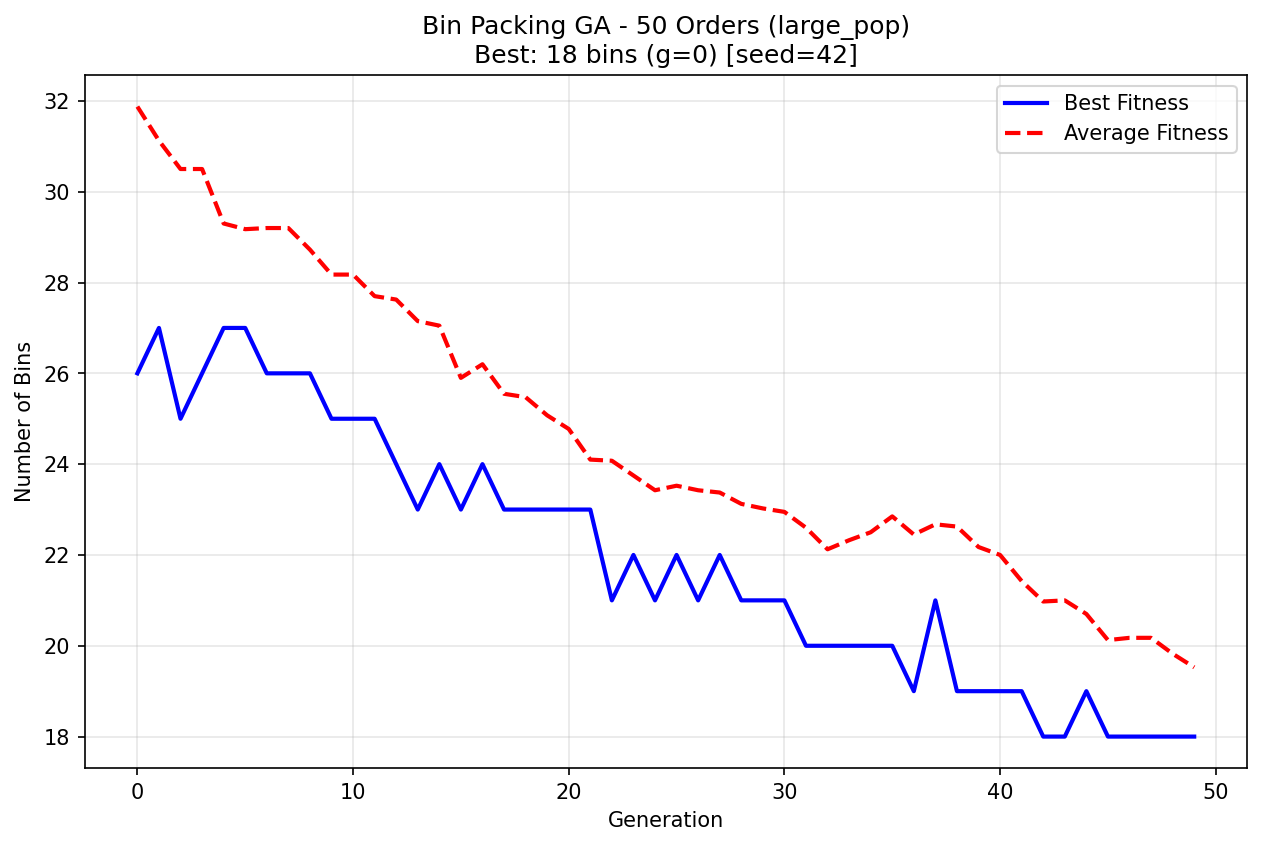
\includegraphics[width=\textwidth]{bpp_50items_large_pop_seed42.png}
    \caption{Large population: 50 orders}
    \label{fig:large_pop_50}
\end{minipage}\hfill
\begin{minipage}{0.48\textwidth}
    \centering
    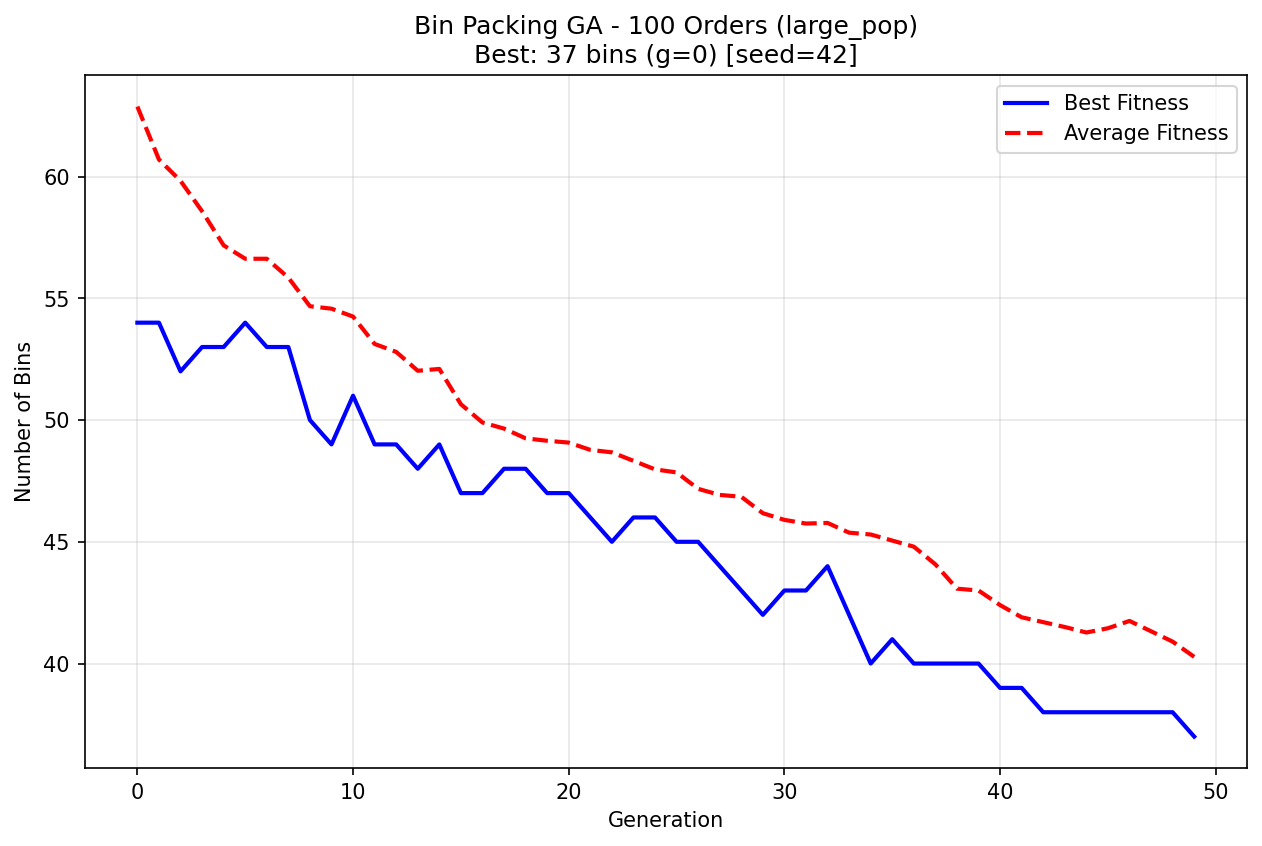
\includegraphics[width=\textwidth]{bpp_100items_large_pop_seed42.png}
    \caption{Large population: 100 orders}
    \label{fig:large_pop_100}
\end{minipage}
\end{figure}

% Short run
\begin{figure}[htbp]
\begin{minipage}{0.48\textwidth}
    \centering
    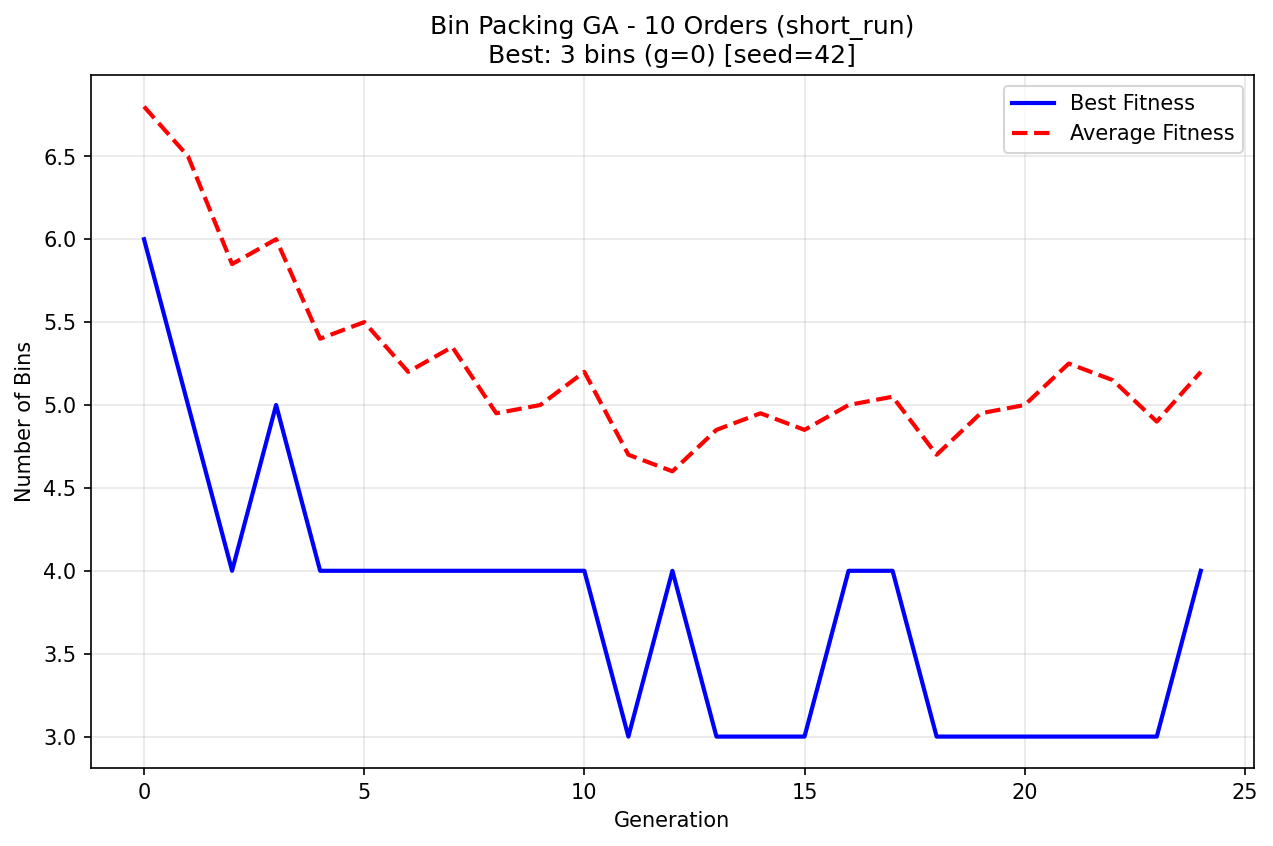
\includegraphics[width=\textwidth]{bpp_10items_short_run_seed42.png}
    \caption{Short run: 10 orders}
    \label{fig:short_run_10}
\end{minipage}\hfill
\begin{minipage}{0.48\textwidth}
    \centering
    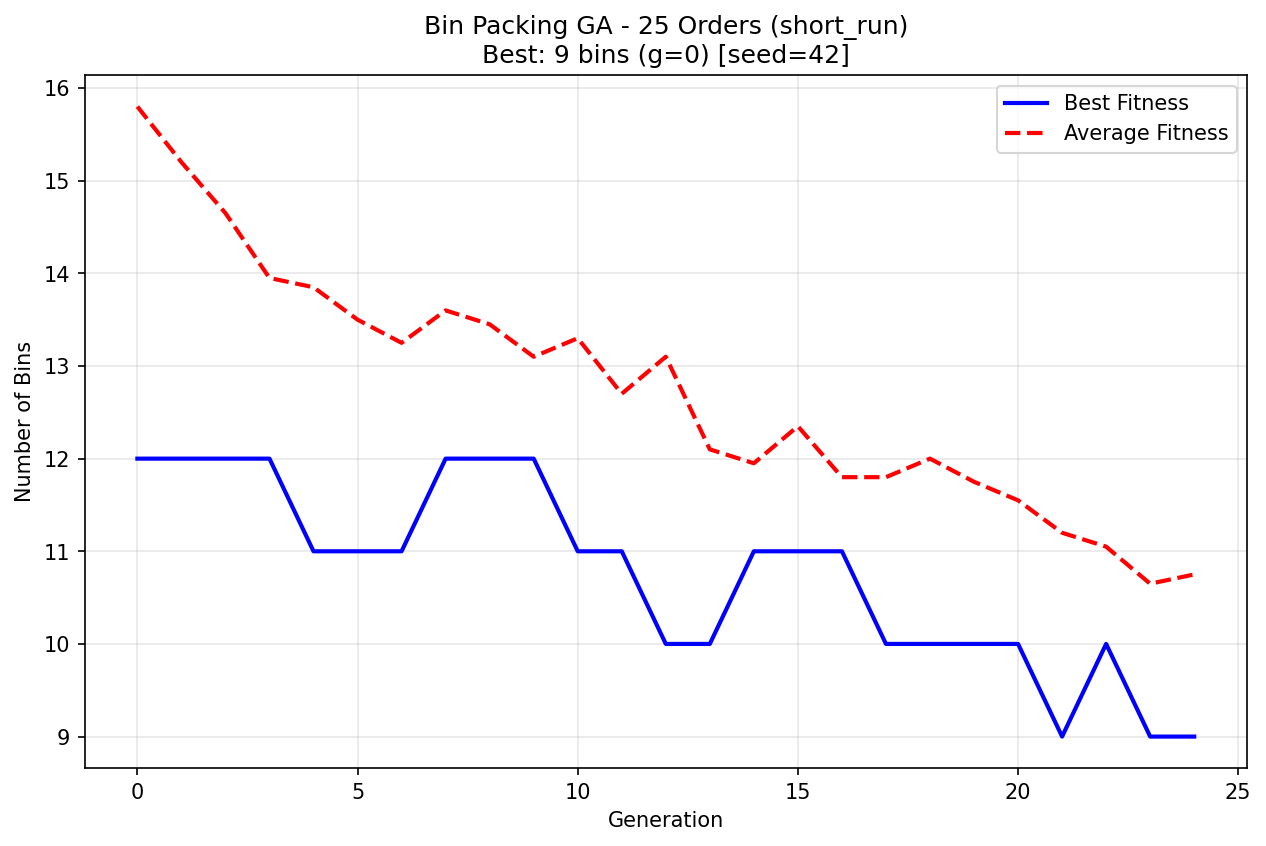
\includegraphics[width=\textwidth]{bpp_25items_short_run_seed42.png}
    \caption{Short run: 25 orders}
    \label{fig:short_run_25}
\end{minipage}
\end{figure}

\begin{figure}[htbp]
\begin{minipage}{0.48\textwidth}
    \centering
    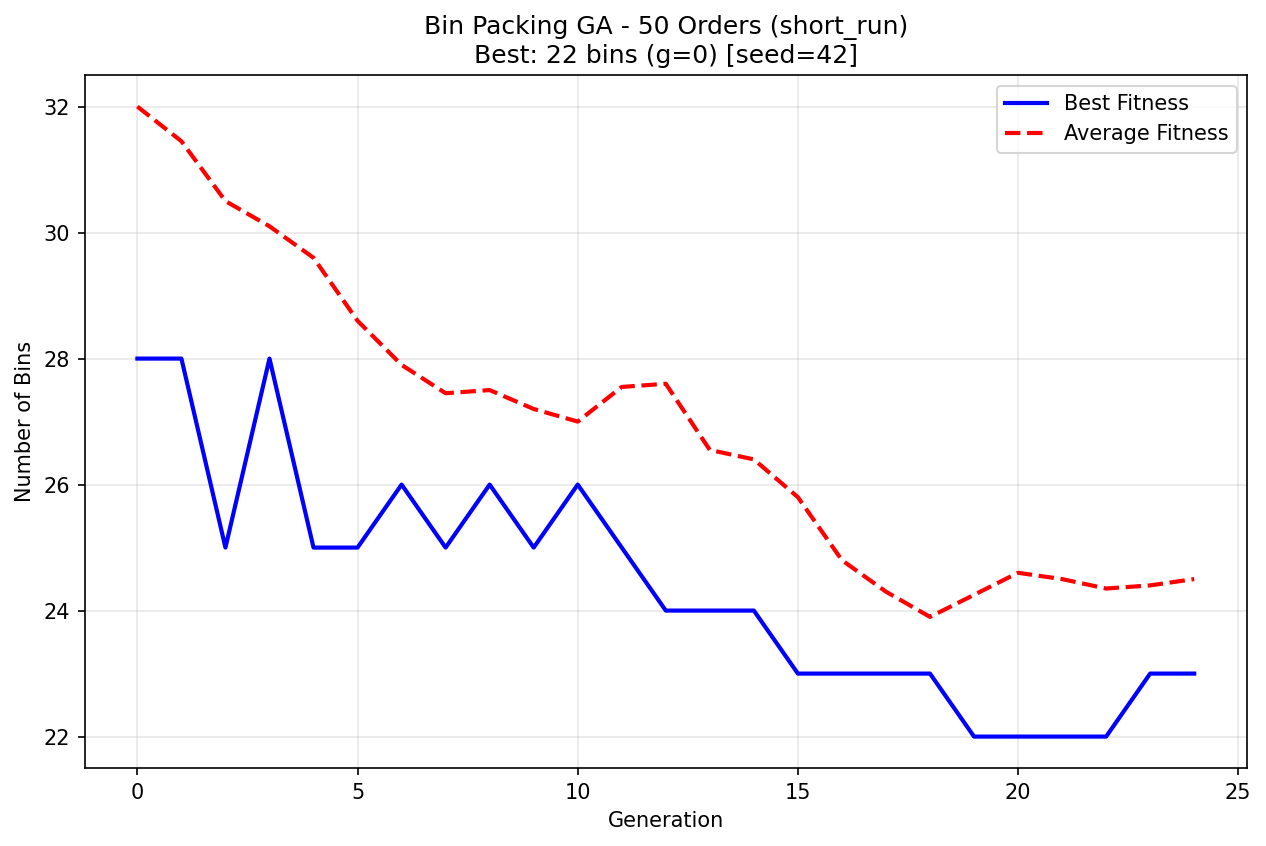
\includegraphics[width=\textwidth]{bpp_50items_short_run_seed42.png}
    \caption{Short run: 50 orders}
    \label{fig:short_run_50}
\end{minipage}\hfill
\begin{minipage}{0.48\textwidth}
    \centering
    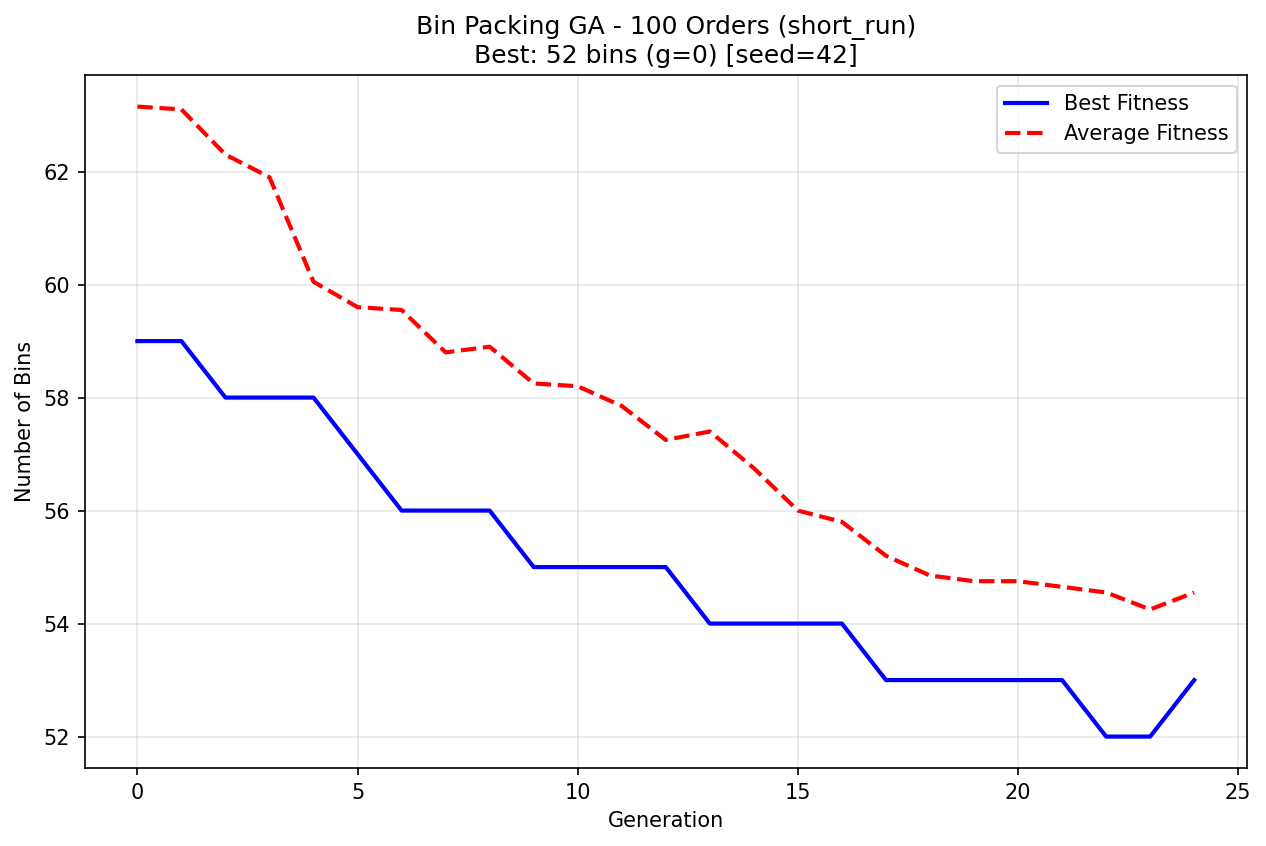
\includegraphics[width=\textwidth]{bpp_100items_short_run_seed42.png}
    \caption{Short run: 100 orders}
    \label{fig:short_run_100}
\end{minipage}
\end{figure}

% Long run
\begin{figure}[htbp]
\begin{minipage}{0.48\textwidth}
    \centering
    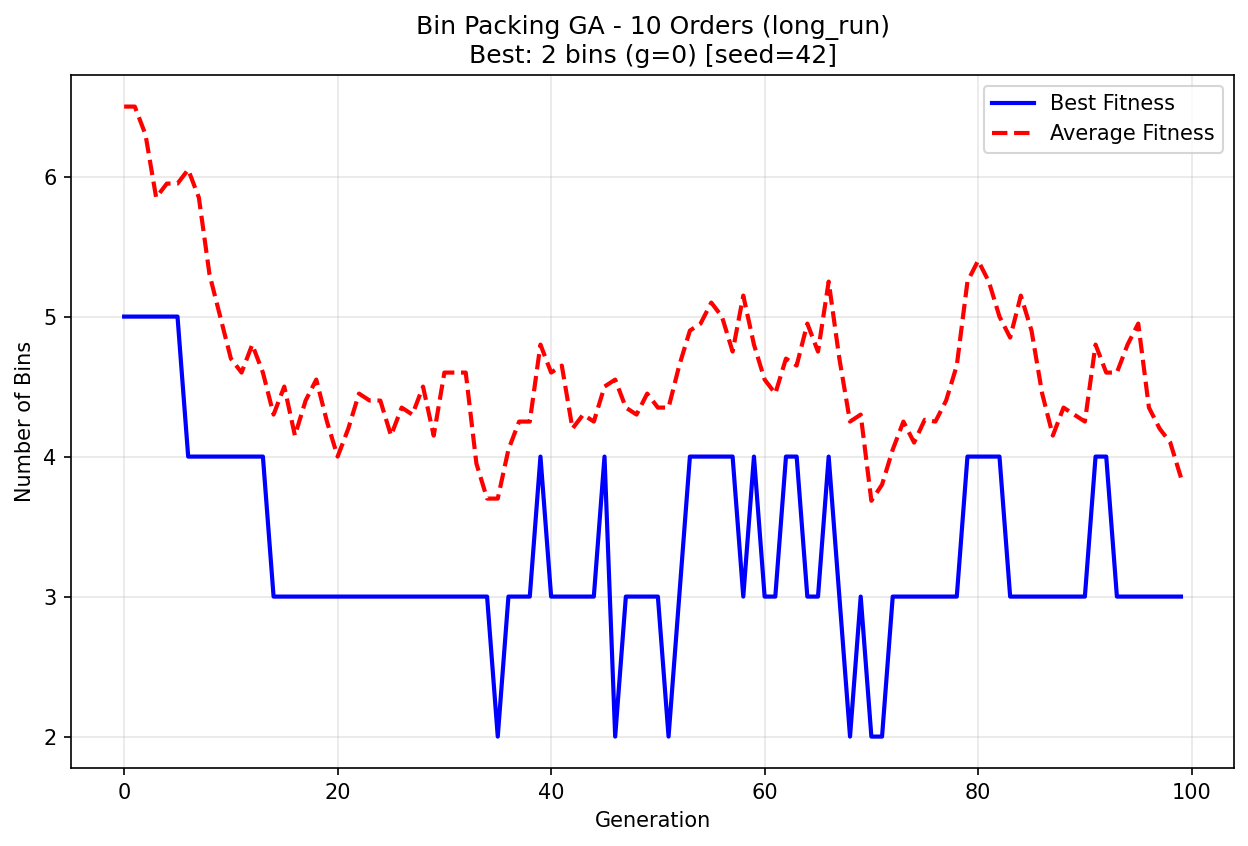
\includegraphics[width=\textwidth]{bpp_10items_long_run_seed42.png}
    \caption{Long run: 10 orders}
    \label{fig:long_run_10}
\end{minipage}\hfill
\begin{minipage}{0.48\textwidth}
    \centering
    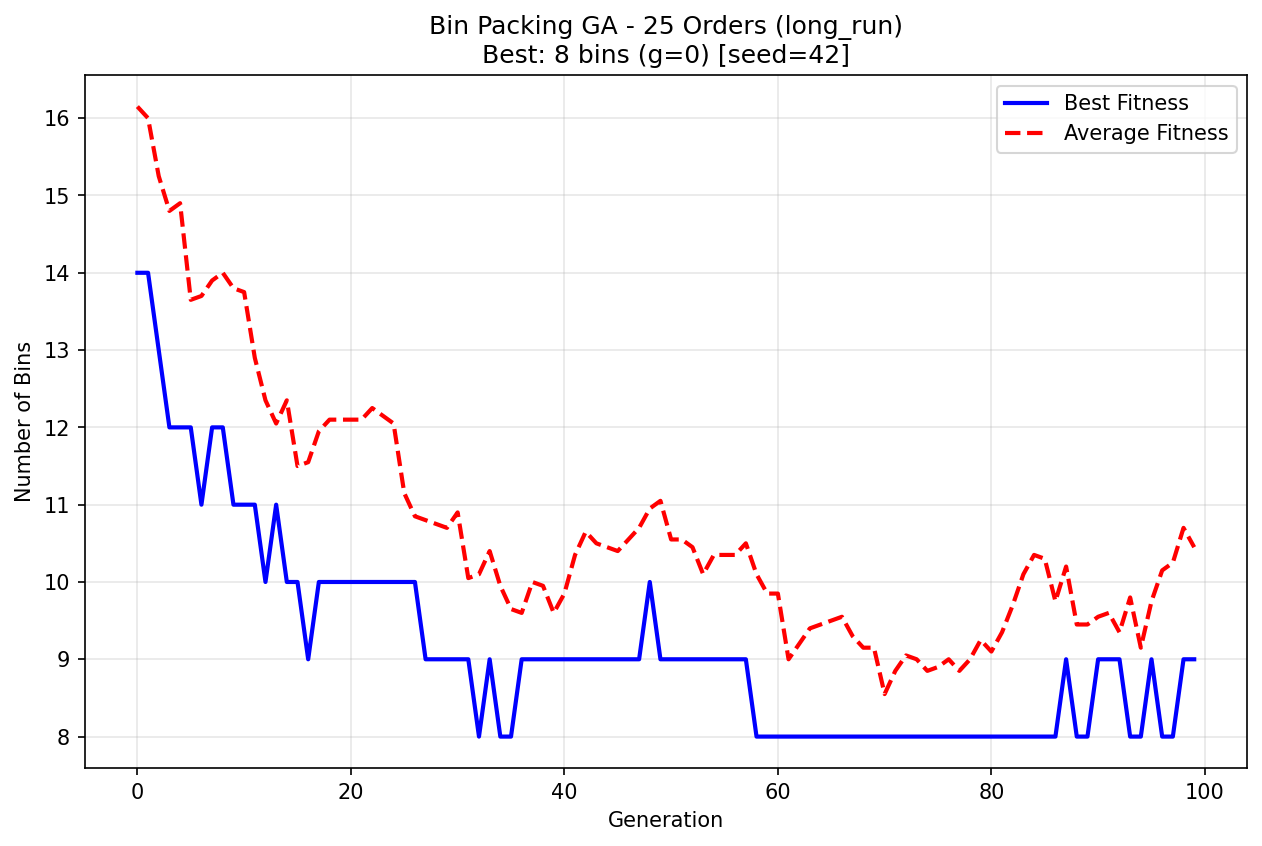
\includegraphics[width=\textwidth]{bpp_25items_long_run_seed42.png}
    \caption{Long run: 25 orders}
    \label{fig:long_run_25}
\end{minipage}
\end{figure}

\begin{figure}[htbp]
\begin{minipage}{0.48\textwidth}
    \centering
    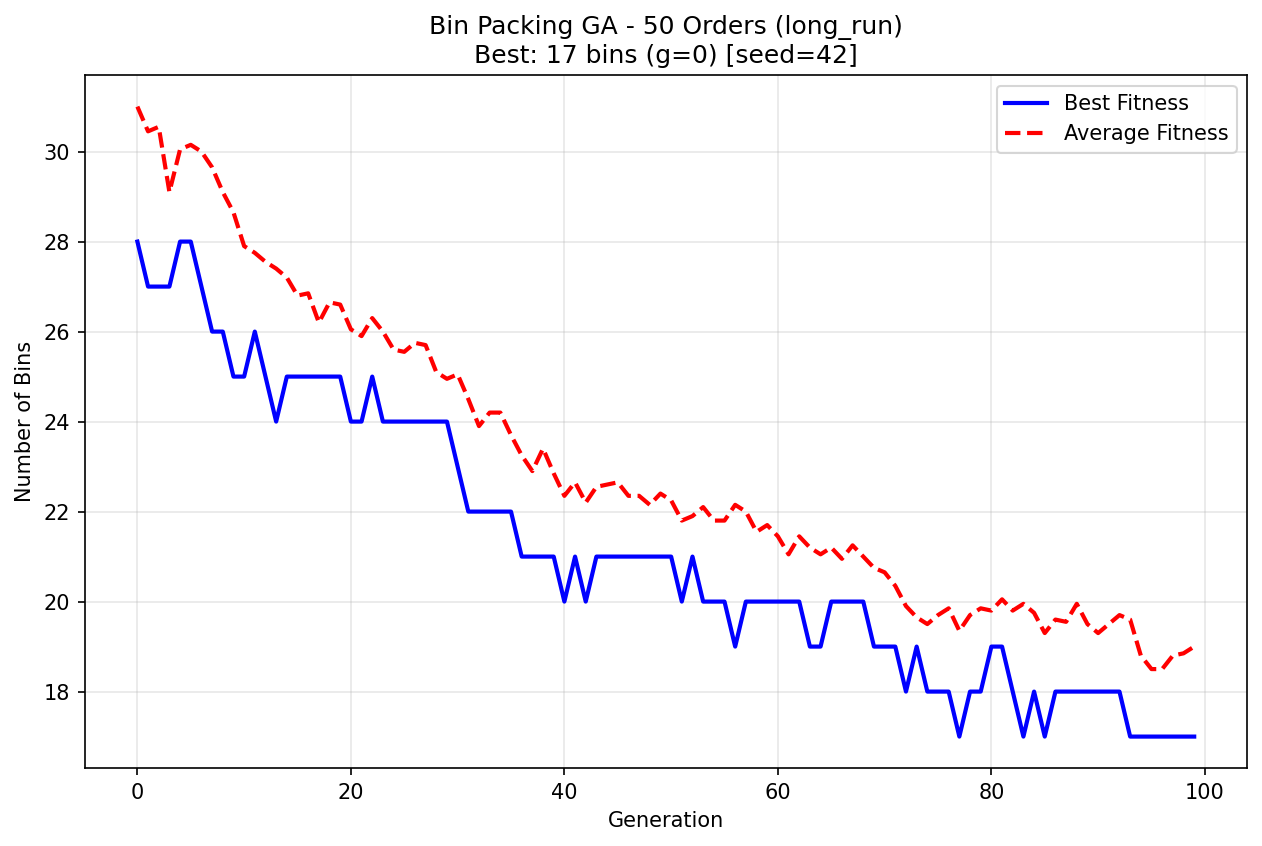
\includegraphics[width=\textwidth]{bpp_50items_long_run_seed42.png}
    \caption{Long run: 50 orders}
    \label{fig:long_run_50}
\end{minipage}\hfill
\begin{minipage}{0.48\textwidth}
    \centering
    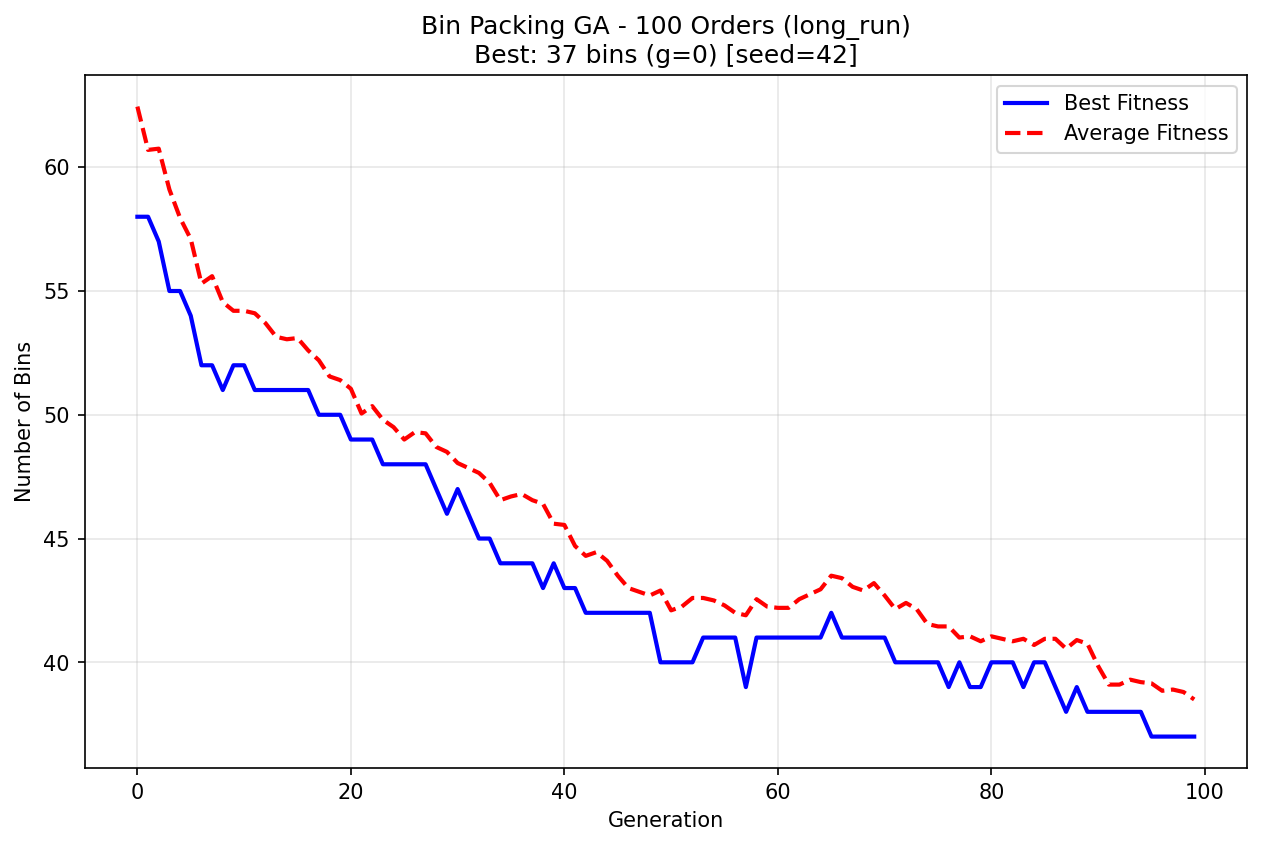
\includegraphics[width=\textwidth]{bpp_100items_long_run_seed42.png}
    \caption{Long run: 100 orders}
    \label{fig:long_run_100}
\end{minipage}
\end{figure}

\subsection{Best Solutions}

Table \ref{tab:best_solutions} summarizes the best solutions found across all configurations tested with seed 42.

\begin{table}[htbp]
\centering
\caption{Best solutions achieved for each configuration}
\label{tab:best_solutions}
\begin{tabular}{|l|c|c|c|c|}
\hline
\textbf{Configuration} & \textbf{10 orders} & \textbf{25 orders} & \textbf{50 orders} & \textbf{100 orders} \\
\hline
Baseline (pop=20, gen=50) & 3 & 7 & 18 & 42 \\
Small pop (pop=10, gen=50) & 2 & 8 & 20 & 43 \\
Large pop (pop=40, gen=50) & 2 & 7 & 18 & 37 \\
Short run (pop=20, gen=25) & 3 & 9 & 22 & 52 \\
Long run (pop=20, gen=100) & 2 & 8 & 17 & 37 \\
\hline
\end{tabular}
\end{table}

The following tables detail the bin-wise packing configurations for the baseline solutions:

\begin{table}[htbp]
\centering
\caption{Baseline packing configuration for 10 orders}
\label{tab:baseline10}
\begin{tabular}{|c|l|r|}
\hline
\textbf{Bin} & \textbf{Items (weights in kg)} & \textbf{Total (kg)} \\
\hline
3 & \#1(1.49), \#4(1.60), \#8(0.18) & 3.27 \\
\hline
6 & \#0(1.22), \#3(1.57), \#5(1.19), \#6(1.89), \#9(0.60) & 6.47 \\
\hline
9 & \#2(0.60), \#7(0.12) & 0.72 \\
\hline
\end{tabular}
\end{table}

\begin{table}[htbp]
\centering
\caption{Baseline packing configuration for 25 orders}
\label{tab:baseline25}
\begin{tabular}{|c|l|r|}
\hline
\textbf{Bin} & \textbf{Items (weights in kg)} & \textbf{Total (kg)} \\
\hline
0 & \#17(0.23), \#20(1.40), \#23(1.15) & 2.78 \\
\hline
3 & \#7(0.11), \#14(1.38), \#22(1.65) & 3.14 \\
\hline
4 & \#13(0.06), \#16(0.83) & 0.89 \\
\hline
17 & \#8(1.94), \#9(0.88) & 2.82 \\
\hline
19 & \#1(0.57), \#2(1.23), \#3(1.79), \#5(1.29), \#6(0.50), \#19(1.63) & 7.01 \\
\hline
21 & \#0(1.87), \#10(1.73), \#15(0.35) & 3.96 \\
\hline
22 & \#4(1.28), \#11(1.01), \#12(1.08), \#18(1.98), \#21(1.15), \#24(0.39) & 6.90 \\
\hline
\end{tabular}
\end{table}

\begin{table}[htbp!]
\centering
\caption{Baseline packing configuration for 50 orders}
\label{tab:baseline50}
\begin{tabular}{|c|l|r|}
\hline
\textbf{Bin} & \textbf{Items (weights in kg)} & \textbf{Total (kg)} \\
\hline
1 & \#2(0.30), \#6(1.75), \#40(0.17) & 2.21 \\
\hline
9 & \#13(1.07), \#15(1.38), \#48(0.90) & 3.35 \\
\hline
10 & \#26(1.41) & 1.41 \\
\hline
14 & \#0(1.67), \#9(1.92), \#12(1.59), \#35(0.34), \#46(0.92), \#49(0.54) & 6.98 \\
\hline
15 & \#3(1.44), \#44(1.73) & 3.18 \\
\hline
17 & \#19(1.97), \#21(1.96) & 3.93 \\
\hline
20 & \#5(1.82), \#37(1.69) & 3.51 \\
\hline
21 & \#1(0.93), \#20(1.67), \#28(0.81), \#42(0.41), \#43(0.70) & 4.52 \\
\hline
23 & \#22(0.46), \#25(0.21) & 0.67 \\
\hline
31 & \#31(0.30) & 0.30 \\
\hline
32 & \#14(1.39), \#27(1.78) & 3.17 \\
\hline
34 & \#17(0.19), \#18(0.92), \#23(1.36), \#33(1.82) & 4.28 \\
\hline
36 & \#30(0.58) & 0.58 \\
\hline
37 & \#4(0.47), \#11(1.46) & 1.93 \\
\hline
39 & \#29(0.98), \#34(1.94), \#39(1.44), \#41(0.71), \#47(1.91) & 6.99 \\
\hline
41 & \#24(0.08), \#32(1.08), \#36(1.30), \#45(0.18) & 2.64 \\
\hline
48 & \#10(0.65), \#16(1.75) & 2.40 \\
\hline
49 & \#7(0.58), \#8(1.52), \#38(0.96) & 3.06 \\
\hline
\end{tabular}
\end{table}

\begin{table}[htbp!]
\centering
\caption{Baseline packing configuration for 100 orders}
\label{tab:baseline100}
\begin{tabular}{|c|l|r|}
\hline
\textbf{Bin} & \textbf{Items (weights in kg)} & \textbf{Total (kg)} \\
\hline
1 & \#71(0.75), \#94(0.78) & 1.53 \\
\hline
4 & \#60(1.30) & 1.30 \\
\hline
7 & \#3(1.65), \#20(0.70), \#69(1.74), \#74(0.67) & 4.77 \\
\hline
8 & \#1(0.50), \#34(1.23) & 1.74 \\
\hline
12 & \#23(1.78) & 1.78 \\
\hline
17 & \#14(1.73), \#28(1.66), \#58(0.31) & 3.71 \\
\hline
20 & \#65(0.60) & 0.60 \\
\hline
21 & \#67(0.51), \#84(1.94), \#96(0.43) & 2.88 \\
\hline
29 & \#38(0.34), \#73(1.49), \#80(1.33) & 3.17 \\
\hline
31 & \#21(1.40), \#68(0.58) & 1.98 \\
\hline
34 & \#22(1.56), \#35(0.94) & 2.50 \\
\hline
36 & \#55(0.01) & 0.01 \\
\hline
37 & \#0(1.49), \#47(1.99), \#49(0.87), \#54(0.47), \#64(1.92) & 6.74 \\
\hline
42 & \#42(1.95), \#70(1.01), \#88(0.25) & 3.21 \\
\hline
44 & \#56(0.88), \#61(1.77) & 2.65 \\
\hline
46 & \#11(0.31), \#19(0.10), \#75(1.55), \#78(1.02), \#91(1.40), \#92(0.07) & 4.45 \\
\hline
49 & \#16(1.64), \#53(0.09), \#63(0.92) & 2.64 \\
\hline
51 & \#29(0.17), \#89(1.73) & 1.91 \\
\hline
52 & \#13(1.51), \#46(1.07) & 2.58 \\
\hline
53 & \#18(0.35), \#39(1.07) & 1.42 \\
\hline
55 & \#27(1.56), \#52(1.66), \#72(1.18) & 4.40 \\
\hline
57 & \#12(0.33), \#40(1.25), \#43(0.28), \#85(1.46) & 3.32 \\
\hline
59 & \#24(0.03) & 0.03 \\
\hline
61 & \#44(0.79), \#57(1.98) & 2.77 \\
\hline
62 & \#10(1.37), \#51(0.53), \#82(0.92), \#83(0.89) & 3.71 \\
\hline
66 & \#31(1.12), \#45(1.80) & 2.92 \\
\hline
68 & \#7(1.81), \#9(0.21), \#37(1.26), \#95(1.82) & 5.11 \\
\hline
69 & \#59(1.73), \#79(1.91), \#99(0.12) & 3.76 \\
\hline
71 & \#33(0.33), \#90(0.68), \#98(0.61) & 1.63 \\
\hline
77 & \#25(0.26), \#26(0.71), \#50(1.29) & 2.26 \\
\hline
78 & \#4(1.95) & 1.95 \\
\hline
81 & \#15(0.05), \#77(0.71) & 0.77 \\
\hline
82 & \#6(0.63), \#17(1.64) & 2.28 \\
\hline
83 & \#30(1.28) & 1.28 \\
\hline
85 & \#81(0.95), \#93(0.01) & 0.97 \\
\hline
86 & \#32(1.45), \#36(0.85) & 2.29 \\
\hline
89 & \#8(0.16), \#76(0.86) & 1.01 \\
\hline
90 & \#41(0.47), \#62(0.46), \#87(1.37) & 2.30 \\
\hline
91 & \#48(1.27) & 1.27 \\
\hline
93 & \#2(1.97), \#66(0.74) & 2.71 \\
\hline
95 & \#86(1.87), \#97(0.55) & 2.43 \\
\hline
97 & \#5(0.52) & 0.52 \\
\hline
\end{tabular}
\end{table}

\section{Q5: Analysis and Comparison}

\subsection{Convergence Analysis}

Performance varied significantly across configurations and problem sizes. Testing with seed 42 revealed clear patterns.

For the smallest problem (10 orders), multiple configurations found 2-bin solutions, including the small population (10 individuals) and long run (100 generations). Small problems proved easy to solve regardless of parameter settings.

Population size mattered more for larger problems. With 100 orders, the small population (10 individuals) needed 43 bins versus the baseline's 42, while the large population (40 individuals) achieved 37 bins - a significant improvement. More diversity helped on complex problems.

Generation count showed similar effects. Short runs (25 generations) performed poorly, especially on large problems—using 52 bins for 100 orders compared to 42 for the baseline. Long runs (100 generations) performed best overall, achieving 17 bins for 50 orders and 37 bins for 100 orders.

Both population size and generation count improved solution quality, with larger problems benefiting most from increased resources in either dimension.

\subsection{Feasible Solution Analysis}

All configurations found feasible solutions (g=0) from generation 0 across all problem instances. This was expected given the problem parameters: with items weighing 0-2 kg and bins holding 10 kg, random initialization rarely produces overloaded bins.

Since each of N items can be assigned to any of N bins, items tend to spread out during random initialization. Even when multiple items land in the same bin, reaching the 10 kg limit requires at least 5 items, which is unlikely when items distribute randomly across many bins.

As a result, the genetic algorithm focused entirely on minimizing the number of bins used rather than finding feasible solutions. The constraint handling mechanisms in the tournament selection were implemented but never needed, as no infeasible solutions appeared during evolution. This shows that for bin packing with generous capacity relative to item size, the challenge is optimization, not constraint satisfaction.

\section{Conclusion}
This study successfully implemented...

\end{document}